\documentclass[a4paper, 12pt]{article}
\usepackage{dirtree}
%\usepackage{cite}
\usepackage[utf8]{inputenc}
\usepackage{listings}
\usepackage{bm}
\usepackage{pdfpages}
\usepackage{fancyhdr}
\usepackage[colorlinks, citecolor=black, urlcolor=blue, bookmarks=false, hypertexnames=true]{hyperref}
\usepackage{biblatex}
\addbibresource{bibilo.bib}
\usepackage{tocloft}
%\renewcommand{\cftsecleader}{\cftdotfill{\cftdotsep}}
%\renewcommand{\cftsecpagefont}{}% Remove \bfseries from section titles' page in ToC
\usepackage{verbatim}
\usepackage{tcolorbox}
\usepackage{amsmath}
\usepackage{amssymb}
\usepackage[utf8]{inputenc}
%\newcommand\logoPath{TU-logo.png}
%\newcommand\logoFileName{TU-logo}
%\newcommand\logoScaleFactor{0.7}
%\usepackage{epigraph}
\usepackage{graphicx}
\usepackage{setspace}
\usepackage{afterpage}
\usepackage{tikz}
\usepackage{amsthm}
\usetikzlibrary{shapes,arrows, positioning}
\usepackage{abstract}
\renewcommand{\abstractnamefont}{\normalfont\large\bfseries}
\newcommand\PROJECTNAME{Geocold}
%\hypersetup{linkbordercolor=black}

\newtheorem{definition}{Definition}


\begin{document}
\graphicspath{\logoPath}
\renewcommand*\contentsname{Table Of Contents}
\newcommand\myemptypage{
		\null
		\thispagestyle{empty}
		\addtocounter{page}{-1}
		\newpage
}

\lstset{language=C++,
		tabsize=3,
				frame=tb,
                basicstyle=\ttfamily,
                keywordstyle=\color{blue}\ttfamily,
                stringstyle=\color{red}\ttfamily,
                commentstyle=\color{green}\ttfamily,
                morecomment=[l][\color{magenta}]{\#}
}
%\lstdefinestyle{mystyle}{frame=tb,
%						language=C++,
%						tabsize=3,
%						numbersep=5pt}

%\lstset{style=mystyle}
\begin{titlepage}
  \begin{center}
      \textbf{
      	  \begin{huge}Project Proposal:\\ \end{huge}
      	  \begin{huge}
      	  \PROJECTNAME \\
			Ray Tracer (Differentiable?) in C++
			\end{huge}}\\
    \vspace{0.5\baselineskip}
    {\Large Authors:  Prakash Chaulagain, Nishar Arjyal, and Pramish Paudel}\\
   	\Large{Roll Numbers: 076BCT045, 076BCT042, 076BCT047} \\
   	\vspace{0.5\baselineskip}
    \centering
      Submitted to the Department of
      Electronics and Computer Engineering
      in Partial Fulfillment of the Requirements of the 3rd Year \textbf{Computer Graphics} Course  
    at 	\\
    {\Large Pulchowk Campus }\\
    {\Large IOE, Tribhuwan University}\\
    \vspace{0.3\baselineskip}
    \today\\
  \end{center}
  \vspace{2\baselineskip}
  {
  \raggedright
		Accepted by: \dotfill

  \raggedleft
  \vspace{1\baselineskip}
  Mr. Basanta Joshi\\
  Assistant Professor at \\
  The Department of Electronics and Computer Engineering\\
  }
  \vspace{2\baselineskip}	
	 Date of Submission: \today \\
  	Expected Date of Completion: July, 2022 
\end{titlepage}
\newpage
\begin{center}
	{\large \textbf{\PROJECTNAME}}\\
	by
	{Prakash Chaulagain, Nishar Arjyal, and Pramish Paudel}\\
	\vspace{0.2\baselineskip}
	\begin{spacing}{0.8}
	{Submitted to the Department of Electronics and Computer Engineering \\
	on \today \\ in Partial Fulfillment of the Requirements for the 3rd Year 
	Computer Graphics Course in Computer Engineering}\\
	\end{spacing}
\end{center}
\begin{abstract}
	Ray tracing has a rich history in the history of computing and computer 
	graphics. With this manuscript, we propose to build an offline ray tracing software using 
	the Vulkan graphics/compute library in C++. Our renderer is supposed to 
	work generically, as in take as input any file containing geometric data,
	perform a mesh render pass in order to render a mesh of the described 
	scene and then perform ray tracing with a separate pass. In this paper, we cover 
	the mathematical principles that we follow as we build our ray tracing software.
\end{abstract}

\newpage

\tableofcontents
\newpage

\begin{section}{Acknowledgement}
	Our project idea is the product of excellent supervision of all of our 
	instructors, most notably our lecturer Mr. Basanta Joshi. We could not 
	have been able to develop interest in computer graphics as a field of study 
	without the constant inspiration provided to us by all of our lecturers and 
	lab instructors and assistants. Some of the credit should also go to 
	the college administration for their efforts in the smooth functioning 
	of all of our classes and labs safely and securely despite the unprecedented 
	times of the pandemic. 
\end{section}

\newpage

\newpage
\pagestyle{fancy}
\fancyhead[C]{\PROJECTNAME}
\fancyhead[L]{}

\renewcommand{\headrulewidth}{0pt}
\renewcommand{\footrulewidth}{0pt}

\begin{tcolorbox}
\begin{center}
	\textit{``He who loves practice without theory is like the sailor who 
	boards ship without a rudder and compass and never knows where he may cast.''} \\
	---Leonardo Da Vinci, 1452-1519
	\end{center}
\end{tcolorbox}

\section{Objectives}
\begin{itemize}
	\item To understand the graphics pipeline.
	\item To become familiar with modern GPU architectures.
	\item To become familiar with GPU programming models and GPU computing (massively parallel computing).
	\item To understand and uncover existing ray tracing techniques.
	\item To gain a degree of familiarity with common graphics and GPU compute APIs, 
	and understand their abstraction mechanisms.
\end{itemize}


\section{Introduction}
	

Rendering is the task of taking a scene composed of many geometric 
objects arranged in 3D space and computing a 2D image that shows the object 
as viewed from a particular viewpoint. The goal of our project \PROJECTNAME~is to create 
a photorealistic renderer by implementing a .obj file loader which then 
creates a mesh of our scene, then finally we implement a ray tracer 
which will correctly color every object in the scene. 
Over the next few sections, we will try and set the mathematical 
basis/principles used in our project and the API that we have attempted to 
design based on those principles.

\section{Theory}
In order to explain the way our ray tracer works, we need to 
set the ground with some basic mathematical 
terms and notations. This will not only give us a more 
technical basis for coming up with a good, mathematically 
correct API, but also help someone using the same 
piece of code to connect the pieces together. The next few of definitions are based on 
Farin(\cite{farin}) and Goldman(\cite{Goldman1985IllicitEI}).

\begin{definition}[Affine Combination in 3D]
	An affine combination of vectors $\bm{x_{1}}, \bm{x_{2}}, \bm{x_{3}}$, 
	$\bm{x_{i}}\in \mathbb{R}^{3}$
	is the linear combination $\sum_{i=1}^{3}\lambda_{j}\bm{x_{i}}$ such that
	$\sum_{j=1}^{3}\lambda_{j}=1$
\end{definition}

\begin{definition}[Affine Map]
	$\Phi:\mathbb{R}^{3}\to \mathbb{R}^{3}$ is an affine map if it leaves affine combinations
	invariant. That is, if
	$$
		\bm{a} = \sum_{j=1}^{3}\lambda_{j}\bm{x_{j}}, \sum_{j=1}^{3}\lambda_{j}=1, \bm{a}, x_{j}\in \mathbb{R}^{3}
	$$
	then, 
	\begin{equation}\label{eqn:affinecomb}
		\Phi(\bm{a}) = \sum_{j=1}^{3}\lambda_{j}\Phi(x_{j}); \Phi(x_{j}), \Phi(\bm{a}) \in \mathbb{R}^{3}.
	\end{equation}
\end{definition}

The  equation\eqref{eqn:affinecomb} specifies the correct way of weighing the 
points $x_{j}$ such that their weighted average is the point $\bm{a}$.

In a given coordinate system, a point $\bm{x}$ is represented in the form of a coordinate triple, 
which we also denote by $\bm{x}$. An affine map now takes the form 
\begin{equation}\label{eqn:affinefunction}
\Phi(\bm{x}) = A\bm{x} + \bm{v}
\end{equation}
The proof that equation\eqref{eqn:affinefunction} is affine is in Farin\cite{farin}.

\subsection{On Points and Vectors}
Goldman (see \cite{Goldman1985IllicitEI}) describes how points and vectors 
are different and ought to be treated differently. Their work also describes 
the way of dealing with their differences.

Points have positions but not direction or length, while vectors have a direction 
and a length. Not all operations that can be applied for vectors can be applied for 
points. Points cannot be added, however addition like operations 
such as an affine combination (also called \textit{barycentric combination}). Although 
we will not go into a comprehensive list of operations that can be 
applied for points and for vectors, we will list (table:\ref{table:pointvec}) out some of the common
operations that are commonly implemented in any legitimate ray tracing API 
(like PBRT\cite{pbrt} and the ones mentioned in Nvidia's Ray Tracing Gems\cite{Haines2019}). 
We denote points with capital letters like $P$ or $Q$, and we denote vectors 
with small boldface letters like $\bm{u}$ or $\bm{v}$.

\setlength{\tabcolsep}{2em}
\begin{table}[htb]
	\centering
	\begin{tabular}{|c c c|}\hline
	Operation & Legal & Undefined	\\ \hline
	Addition & $\bm{u}$+$\bm{v}$(v), P+$\bm{u}$(p) & P+Q \\
	Subtraction & $\bm{u}$-$\bm{v}$(v), P-$\bm{u}$ & $\bm{u}-\bm{P}$\\
	Scalar Multiplication & c.$\bm{v}$(v) & c.P \\
	Dot Product & $\bm{u}.\bm{v}$(scalar) & P.$\bm{u}$, P.Q \\
	Cross Product & $\bm{u}\times \bm{v}$(v) & P $\times$Q, P $\times\bm{u}$\\ \hline
	\end{tabular}
	\caption{Common operations defined for points and vectors. (v in the braces 
	represents vector and p represents point)}
	\label{table:pointvec}
\end{table}

To come up with a decent and mathematically correct ray tracer, it is essential 
that we use the C++ type system to deal with these inherent differences between 
mathematical constructs.

\begin{lstlisting}[caption=Sample code for Point3 and Vec3 types]
	template<typename T>
	struct Vec3; //forward declaration

	template <typename T>
	struct Point3 {
		T x_;
		T y_;
		T z_;
		Point3(T x, T y, T z) noexcept 
		   :x_{x}, 
			y_{y}, 
			z_{z} {}
		
		Point3 operator+(const Vec3<T>& vec) noexcept {
			return Point3<T>{
				x_ + vec.x_,
				y_ + vec.y_,
				z_ + vec.z_
			};
		} //this implements Point3 + Vec3

		Vec3<T> operator-(const Point3& rhs) noexcept {
			return Vec3<T>{
				x_ - rhs.x_,
				y_ - rhs.y_,
				z_ - rhs.z_
			};
		} // Point3 - Point3 -> Vec3 

		Point3<T> operator-(const Vec3<T>& vec) noexcept {
			return Point3<T>{
				x_ - vec.x_,
				y_ - vec.y_,
				z_ - vec.z_
			};
		}
	};

	template <typename T>
	struct Vec3<T> {
		T x_;	
		T y_;	
		T z_;	

		Vec3(T x, T y, T z) noexcept 
			:x_{x}
			,y_{y}
			,z_{z} {}
		
		Vec3<T> operator-() const {
			return Vec3<T>{
				-x_,
				-y_, 
				-z_
			};
		}

		Vec3<T> operator*(T scalar) {
			return Vec3<T>{
				x*scalar,
				y*scalar,
				z*scalar
			};
		}

//other trivial operations like 
//vector addition, 
//subtraction, dot product and cross 
//product are also implemented.
//Vec3 - Point3 is not implemented 
//as it is an invalid operation.
	};
\end{lstlisting}

\subsection{Other Primitives}
\begin{definition}[Normal]
	A surface normal is a vector perpendicular to a surface at a 
	particular position.
\end{definition}

It is necessary to have a separate type for normals as 
they are treated differently to vectors (normals take 
object properties into account). Advanced ray tracers 
(like \cite{pbrt}) also take into account the various
partial derivatives of the surface normal with respect
to the local parametrization of the curve. In 
ray tracing, it is essential to know the normal 
to the surface at which the ray-triangle 
intersection test is satisfied so as to 
compute the direction in which the ray will be reflected next.

\begin{definition}[Ray]
	We represent a ray as a parametric line in \PROJECTNAME.
	If $\bm{a}$ and $\bm{b}$ are two points such that 
	the ray starts at $\bm{a}$ then, the line between 
	$\bm{a}$ and $\bm{b}$ is given by the parametric equation: 
	\begin{equation}
		\bm{r}(t) = (1-t)\bm{a} + t\bm{b}, t\in [0,1]
	\end{equation}
\end{definition}
	This is obviously an affine combination of the points $\bm{a}$ and $\bm{b}$.
	However, on slight modification, we can implement a ray 
	as a linear combination of a point and a vector as such:
	\begin{equation}
		\bm{r}(t) = \bm{a} + t(\bm{b}-\bm{a})
	\end{equation}

	But, we need the parameter $t$ to be in a set interval so
	that we won't have to track the ray farther than we need to
	(upto when the ray passes the ray-triangle intersection test).
	The ray can also not go behind the camera or eye.
	So, we need fields $tmin$ and $tmax$ for our struct.

	\begin{lstlisting}
		struct Ray {
			Point3<float> a;
			float tmin;
			Vec3<T> direction; //b-a
			float tmax;
		}; //ray is left unparametrized
	\end{lstlisting}

	Since most computer graphics projects
	define common camera models, we won't go
	to depth on the camera model for ray tracing in 
	this paper. 

	We will finally end this section with a few words 
	on radiosity and light model.

\subsection{Raidosity and Light Models}
\begin{center}
\begin{figure}
	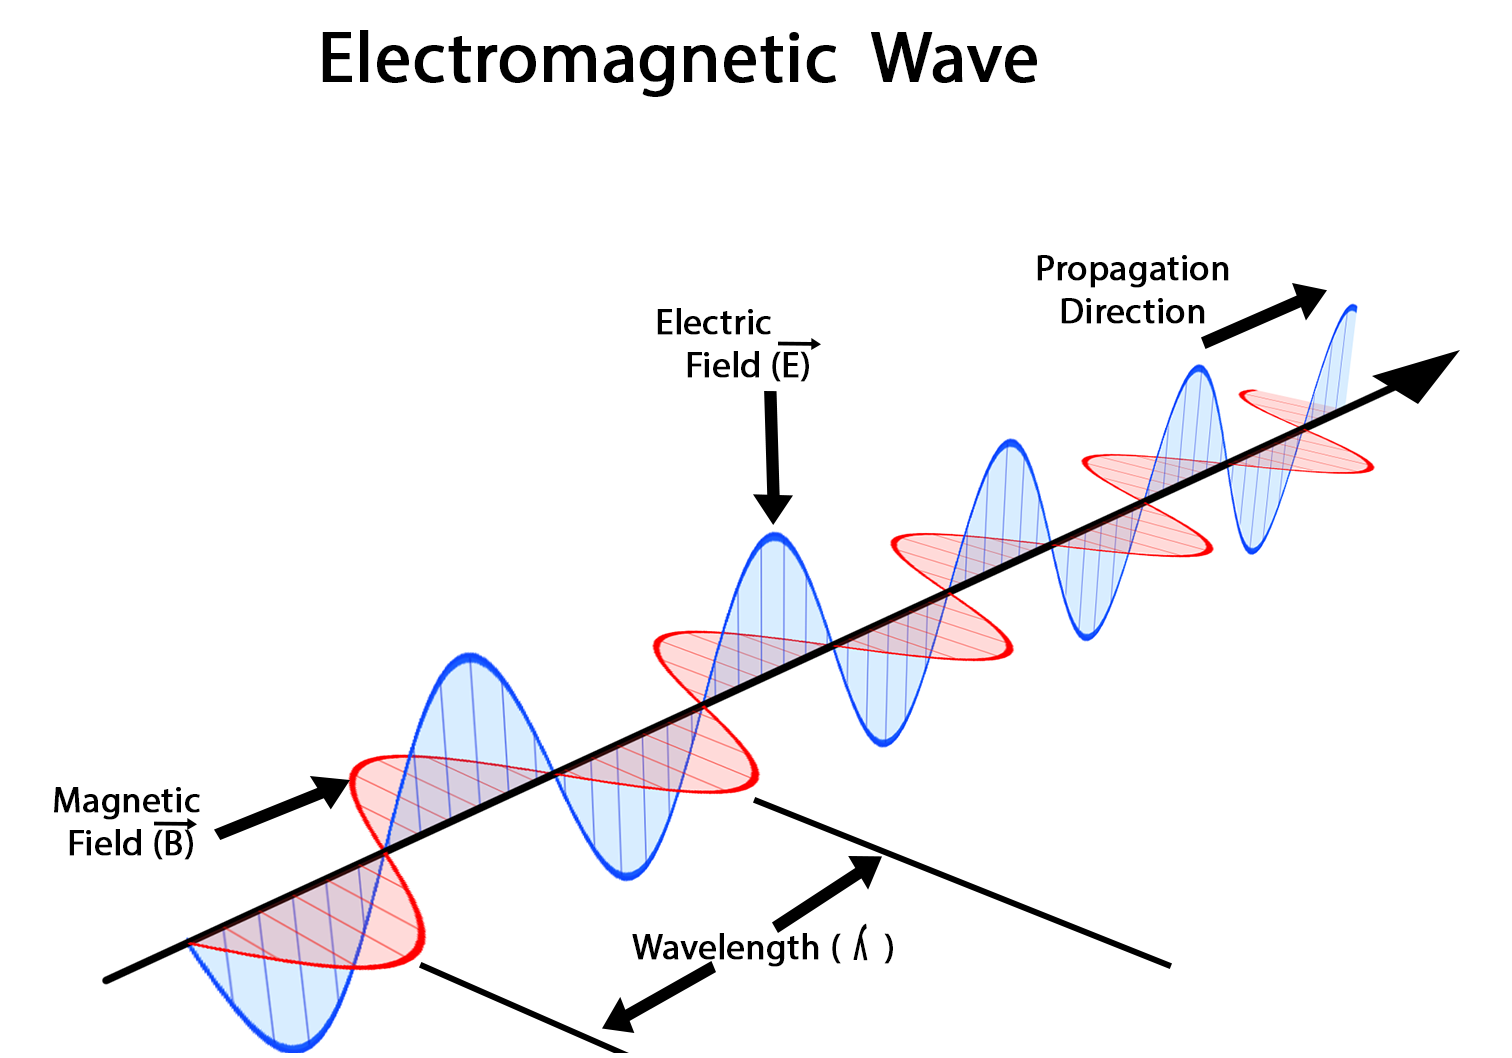
\includegraphics[width=0.6\linewidth, scale=0.8]{lightem.png}
	\centering
	\caption{Light as an electromagnetic wave.}
\end{figure}
\end{center}
Light is an electromagnetic wave that propagates through space. 
A convincing computer model for light would incorporate into it 
the direction of propagation, speed, wave-lenth, amplitude, polarization 
and so on. Although not all of these parameters are incorporated in 
standard ray tracers, ours will be a lightweight one in which we 
shall model light without any polarizability.
The vector form for the law of reflection of light is as follows: 
$$
\bm{\omega}_{r}=\bm{\omega}_{i}-2\bm{n}_{p}(\bm{\omega}_{i}.\bm{n}_{p})
$$

\subsubsection{Whitted Ray Tracing}
Turner Whitted in his paper 'An Improved Illumination Model
For Shaded Display'\cite{whitted} highlighted the use of 
geometric optics in rendering. He improved upon the Phong 
illumination model\cite{Phong1975IlluminationFC} by replacing specular component
in his model by the intensity S of the light coming from the direction of 
specular reflection. His model also accounted for 
transmitted light intensity by adding T term weighted by $k_{t}$ coefficient 
of transmitted light contribution.

\begin{equation}\label{eqn:whittedmodel}
I = I_{a} + k_{d}\sum_{i}^{l}L_{i,d}(\bm{n}.\bm{\omega}_{i}) + k_{s}S + k_{t}T
\end{equation}
where: \\
$I_{a}$ = intensity of ambient component \\
$k_{d}\text{ and } k_{s}$ = diffues and specular coefficients \\ 
$L_{i,d}$ = diffuse intensity of ith light source \\
$\bm{n}$ = equivalent to reflection sharpness in Phong\cite{Phong1975IlluminationFC},
handled by adjusting random perturbations in $\bm{n}$ vector \\
$l$ = number of light sources

S and T intensities depend on previous light hits and hence, must be calculated 
recursively.

\subsection{Measuring Light}
Our ray tracer however, should be able to handle the effect of 
the wavelength of light in the ways it behaves after striking 
a surface/object in the scene. Our 
ray tracer will disregard the spectrums and 
only deal with RGB. First, let's define some terms from radiometry.
A rigorous discussion of the following theory is available in 
Lafortune\cite{Lafortune1995MathematicalMA} and Wojciech Jarosz's Ph.D. 
Dissertation\cite{jarosz08thesis} on the same topic also does an excellent job
at making these ideas clear.

\begin{definition}[Radiant Energy]
Electromagnetic radiations carry energy through space.
The energy carried by a single photon emitted by a source 
of illumination is given by 
$$
	Q = \cfrac{hc}{\lambda}
$$
\end{definition}

\begin{definition}[Radiant Flux]
Radiant Flux or power is defined as the total amount of energy passing 
through a surface or region of space per unit time.
$$
	\Phi = \cfrac{dQ}{dt}
$$
\end{definition}

\begin{definition}[Radiant Flux Density]
	Radiant Flux Density is the radiant flux per unit area at a 
	point on a surface, where the surface could be real or imaginary.
\end{definition}

\begin{center}
\begin{figure}
	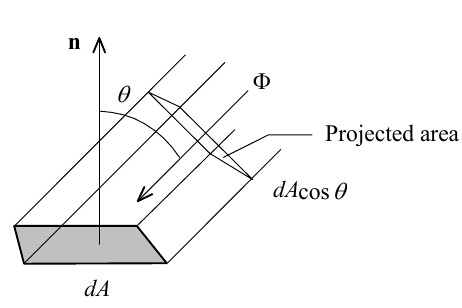
\includegraphics[width=0.8\linewidth, scale=0.6]{raynormal.png}
	\centering
	\caption{Ray of Light Intersecting a surface}
	\label{figure:rayandnormal}
\end{figure}
\end{center}

\begin{center}
\begin{figure}
	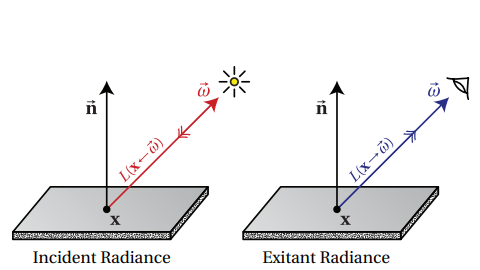
\includegraphics[width=0.8\linewidth, scale=0.6]{incidentradiance.png}
	\centering
	\caption{Incident and Exitant Radiance}
	\label{figure:incidentexitant}
\end{figure}
\end{center}

\begin{definition}[Irradiance E]
	The radiant flux arriving at a surface per unit area 
	is called irradiance. 
	$$
		E = \cfrac{d\Phi}{dA}
	$$
\end{definition}

\begin{definition}[Radiant Exitance M]
	The radiant flux leaving from a surface per unit area 
	is called radiant exitance. 
	$$
		M =  \cfrac{d\Phi}{dA}
	$$
\end{definition}


\begin{definition}[Radiance]
	Imagine an elemental cone to represent a 
	ray that intersects a surface making an 
	angle $\theta$ with the surface normal as in figure~\ref{figure:rayandnormal}.
	The projected area of the ray-surface intersection area $dA$
	is $dAcos\theta$. The radiance is the radiant flux 
	density per unit elemental cone or per unit solid 
	angle $d\omega$. 
	\begin{equation}\label{eqn:radiance}
		L = \cfrac{d^{2} \Phi}{dA cos\theta d\omega} = \cfrac{d^{2}\Phi(\bm{p}, \bm{\omega})}{(\bm{n}_{p}.\bm{\omega})d\bm{\omega}dA(\bm{p})}
	\end{equation}
\end{definition}

We can also integrate equation \eqref{eqn:radiance} over the hemisphere of directions $\Omega$
and area $dA$ to obtain 

$$
\Phi = \int_{A}\int_{\Omega}L(\bm{p}\to \bm{\omega})(\bm{n}_{p}.\bm{\omega})d\bm{\omega}dA(\bm{p})
$$

We can also compute the irradiance and radiant exitance 
using :

\begin{equation}\label{eqn:irradianceradiance}
	E(\bm{p}) = \int_{\Omega}L(\bm{p}\leftarrow \bm{\omega})(\bm{n}_{p}.\bm{\omega})d\bm{\omega} 
\end{equation}
\begin{equation}
	M(\bm{p}) = \int_{\Omega}L(\bm{p}\to \bm{\omega})(\bm{n}_{p}.\bm{\omega})d\bm{\omega} 
\end{equation}

Although in the case of surfaces in general, 
$$
L(\bm{p}\to \bm{\omega}) \neq L(\bm{p}\leftarrow \bm{\omega}) 
$$

In vacuum where photons can propagate unobstructed, all the radiance incident at a 
point from a direction $\bm{\omega}$ will continue on in the form of 
exitant radiance in the direction $-\bm{\omega}$. Because of this, we can form a simple 
relation between exitant and incident radiance at a point. To accomplish, 
we can come up with a ray casting function $\bm{r(\bm{p}, \bm{\omega})} = \bm{p}$'
which returns $\bm{p}$', the point on the closest surface from $\bm{p}$ in the
direction $\bm{\omega}$. Since radiance stays constant in vacuum along a 
straight line, we can say that the incidence radiance at a point $\bm{p}$ from 
direction $\bm{\omega}$ is equal to the outgoing radiance from the closest visible points 
in that direction. That is 
\begin{equation}\label{eqn:inputoutputinvariance}
L(\bm{p}\leftarrow \bm{\omega}) = L(\bm{p}' \to -\bm{\omega})
\end{equation}
Although our ray tracer will not incorporate the effect of participating 
medium on the rays, we will have to take the material properties into 
account as even the most minimal of ray tracers ought to do.

\subsection{Interaction of Light with Surfaces}
\subsubsection{The Bidirectional Reflectance Distribution Function}
If $\bm{\omega}_{i}$ be the incoming direction, and $\bm{\omega}_{0}$ be the outgoing direction, then 
the BRDF($f_{r}$) gives a measure for the amount of radiance impinging at a point $\bm{p}$ along 
a direction $\bm{\omega}_{i}$ that is reflected along $\bm{\omega}_{0}$. Formally, 
\begin{equation}\label{eqn:brdf}
	f_{r}(\bm{\omega}_{i}, \bm{p}, \bm{\omega}_{o}) = \cfrac{dL_{o}(\bm{p}, \bm{\omega}_{o})}{dE(\bm{p},\bm{\omega}_{i})}
	= \cfrac{dL_{o}(\bm{p}, \bm{\omega}_{o})}{L_{i}(\bm{p}, \bm{\omega}_{i})(\bm{n}_{p}.\bm{\omega}_{i})d\bm{\omega}_{i}}
\end{equation}
The last step is obtained from \eqref{eqn:irradianceradiance}.

The information in the BRDF can be used to derive the relationship between incident and reflected 
radiance. By manipulating and then integrating \eqref{eqn:brdf} over all directions, we can derive 
an expression for computing the reflected radiance at a point $\bm{p}$. We also note that 
the total radiance leaving a surface is the sum of the emitted radiance and the reflected radiance and 
also from \eqref{eqn:brdf} we get:
$$
L_{o}(\bm{p}, \bm{\omega}_{o}) = L_{e}(\bm{p}, \bm{\omega}_{o}) + \int_{\Omega_{i}}L_{i}(\bm{p}, \bm{\omega}_{i})
f_{r}(\bm{\omega}_{i}, \bm{p}, \bm{\omega}_{o})|\bm{\omega}_{i}.\bm{n}_{p}|d\bm{\omega}_{i}
$$

Since each incidence radiance corresponds to an outgoing 
radiance, as expressed in equation \eqref{eqn:inputoutputinvariance}, 
and also if $\bm{r}(\bm{p}, \bm{\omega})$ be the ray casting function then the 
gloabal illumination model of the famous rendering equation as 
described by James Kajiya in his paper 'The Rendering Equation'\cite{kajiya}
in hemispheric form: 

\begin{equation}\label{eqn:renderingequation}
L_{o}(\bm{p}, \bm{\omega}_{o}) = L_{e}(\bm{p}, \bm{\omega}_{o}) + \int_{\Omega_{i}}L_{o}(\bm{r}(\bm{p}, -\bm{\omega_{i}}), \bm{\omega}_{i})
f_{r}(\bm{\omega}_{i}, \bm{p}, \bm{\omega}_{o})|\bm{\omega}_{i}.\bm{n}_{p}|d\bm{\omega}_{i}
\end{equation}

Kajiya suggested we follow a Monte Carlo approach 
to computing the equation \eqref{eqn:renderingequation} 
in a method that is now commonly called Path Tracing.

Although several top notch BRDFs exist (notably 
the Cook-Torrance model\cite{cooktorrance}), 
we will be using the Phong distribution: 
$$
f_{r}(\bm{\omega}_{i}, \bm{p}, \bm{\omega}_{o}) = k_{d}\cfrac{1}{\pi}+k_{s}\cfrac{n+2}{2\pi}\text{cos}^{n}\alpha
$$

where $\alpha$ = angle between the reflected ray and ideal specular reflection and 
n is the specular exponent. For preservation of energy, the restriction that $k_{s}+k_{d}\leq 1$
is essential.

\section{Existing Systems}
Several top notch ray tracing APIs already exist 
in the computer graphics world. Vulkan, the graphics 
+ compute API has a ray tracing pipeline in one of 
its extensiosn. Advanced game engines 
like Unity handle ray tracing by themselves 
while other contemporary platform specific
computer graphics APIs like DirectX have their own 
ray tracing pipeline. Obviously for 
physically based rendering the PBRT\cite{pbrt} is 
the best resource for beginners like ourselves to learn.
A more convincing analysis 
of existing ray tracing APIs 
Ours is a simple ray tracer that implements the 
Whitted Ray Tracer Model but we are inclined to 
also have a little support for the Kajiya rendering equation.

\section{System Block Diagram}
\begin{center}
\begin{figure}[htb]
	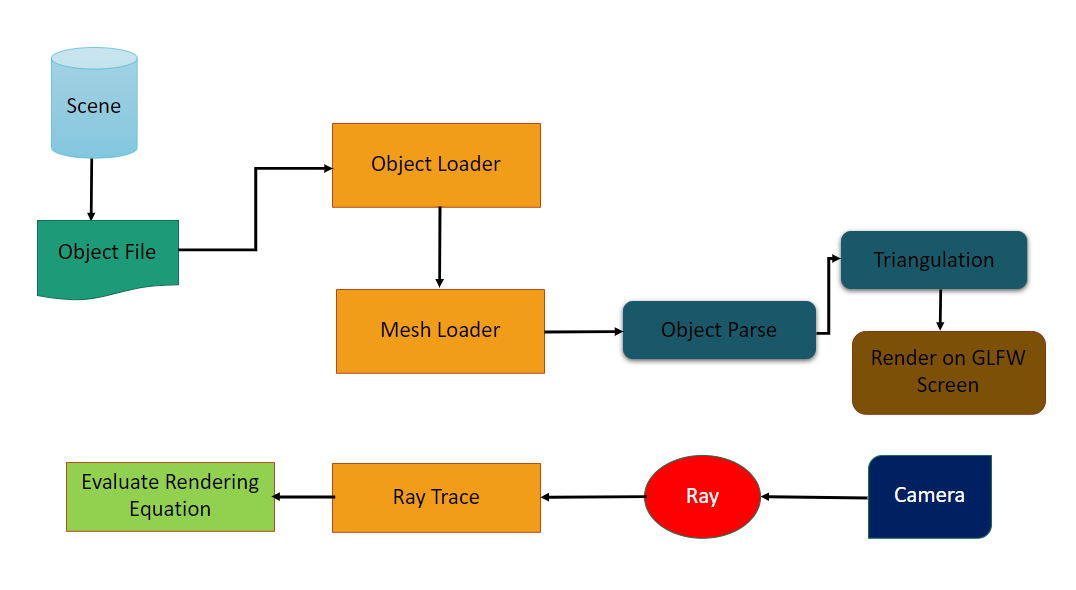
\includegraphics[width=1.2\linewidth, scale=1.2]{massivesizedblockD.png}
	\centering
	\caption{A simple block diagram representing the workings of \PROJECTNAME}
	\label{figure:systemblock}
\end{figure}
\end{center}

\section{Project Schedule}
The work on the project has already begun and we 
wish to finish the work as quickly as we can. 
The project is supposed to be quite a heavy one with 
tons of code for doing physically based rendering 
and also for actually rendering things on the 
screen using graphics APIs. The final project alongside
with a report shall be submitted within the 
allocated time i.e., it should be finished by the end of July.

\newpage
\printbibliography
\end{document}


